\chapter{Configuring and Running the DevOps Pipeline \\
\small{\textit{-- JGa, JGr, CS}}}
\label{Chapter::DevopsPipeline}

This chapter documents the configuration and execution of the DevOps pipeline developed for this project. The pipeline follows the principles of the V-Curve Development Cycle, ensuring that each phase of development is paired with a corresponding validation or verification activity. The primary goal of this pipeline is to automate documentation builds while maintaining traceability, reliability, and early detection of defects.

\section{Issue Tracking}

Issue tracking for this project is handled using GitHub Issues. Issues are used to record bugs, required changes, and enhancement requests. Each issue provides a clear description of the problem or requirement and can be directly linked to commits and workflow executions. This creates traceability from the initial requirement through implementation and verification, aligning with the left and right sides of the V-Curve.

\begin{figure}[h!]
    \centering
    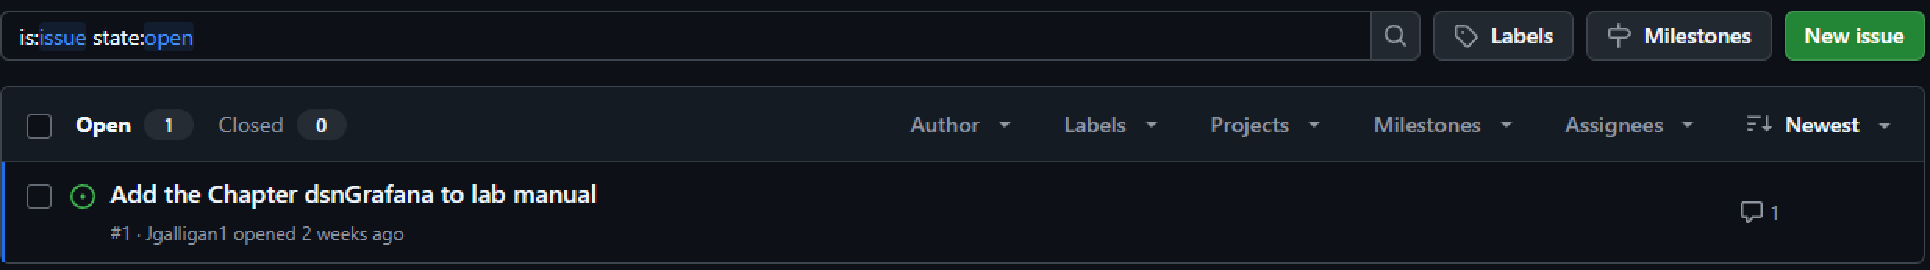
\includegraphics[width=0.9\linewidth]{pdf/a_IssueTracking.pdf}
    \caption{Basic issue tracking}
\end{figure}

\section{Source Control}

Git is used as the source control system for all project artifacts, including LaTeX source files and generated PDFs. Hosting the repository on GitHub allows version history to be preserved and enables automatic triggering of the CI pipeline whenever changes are pushed to the \texttt{master} branch. This ensures that every documented change is immediately validated through the pipeline.

\begin{figure}[h!]
    \centering
    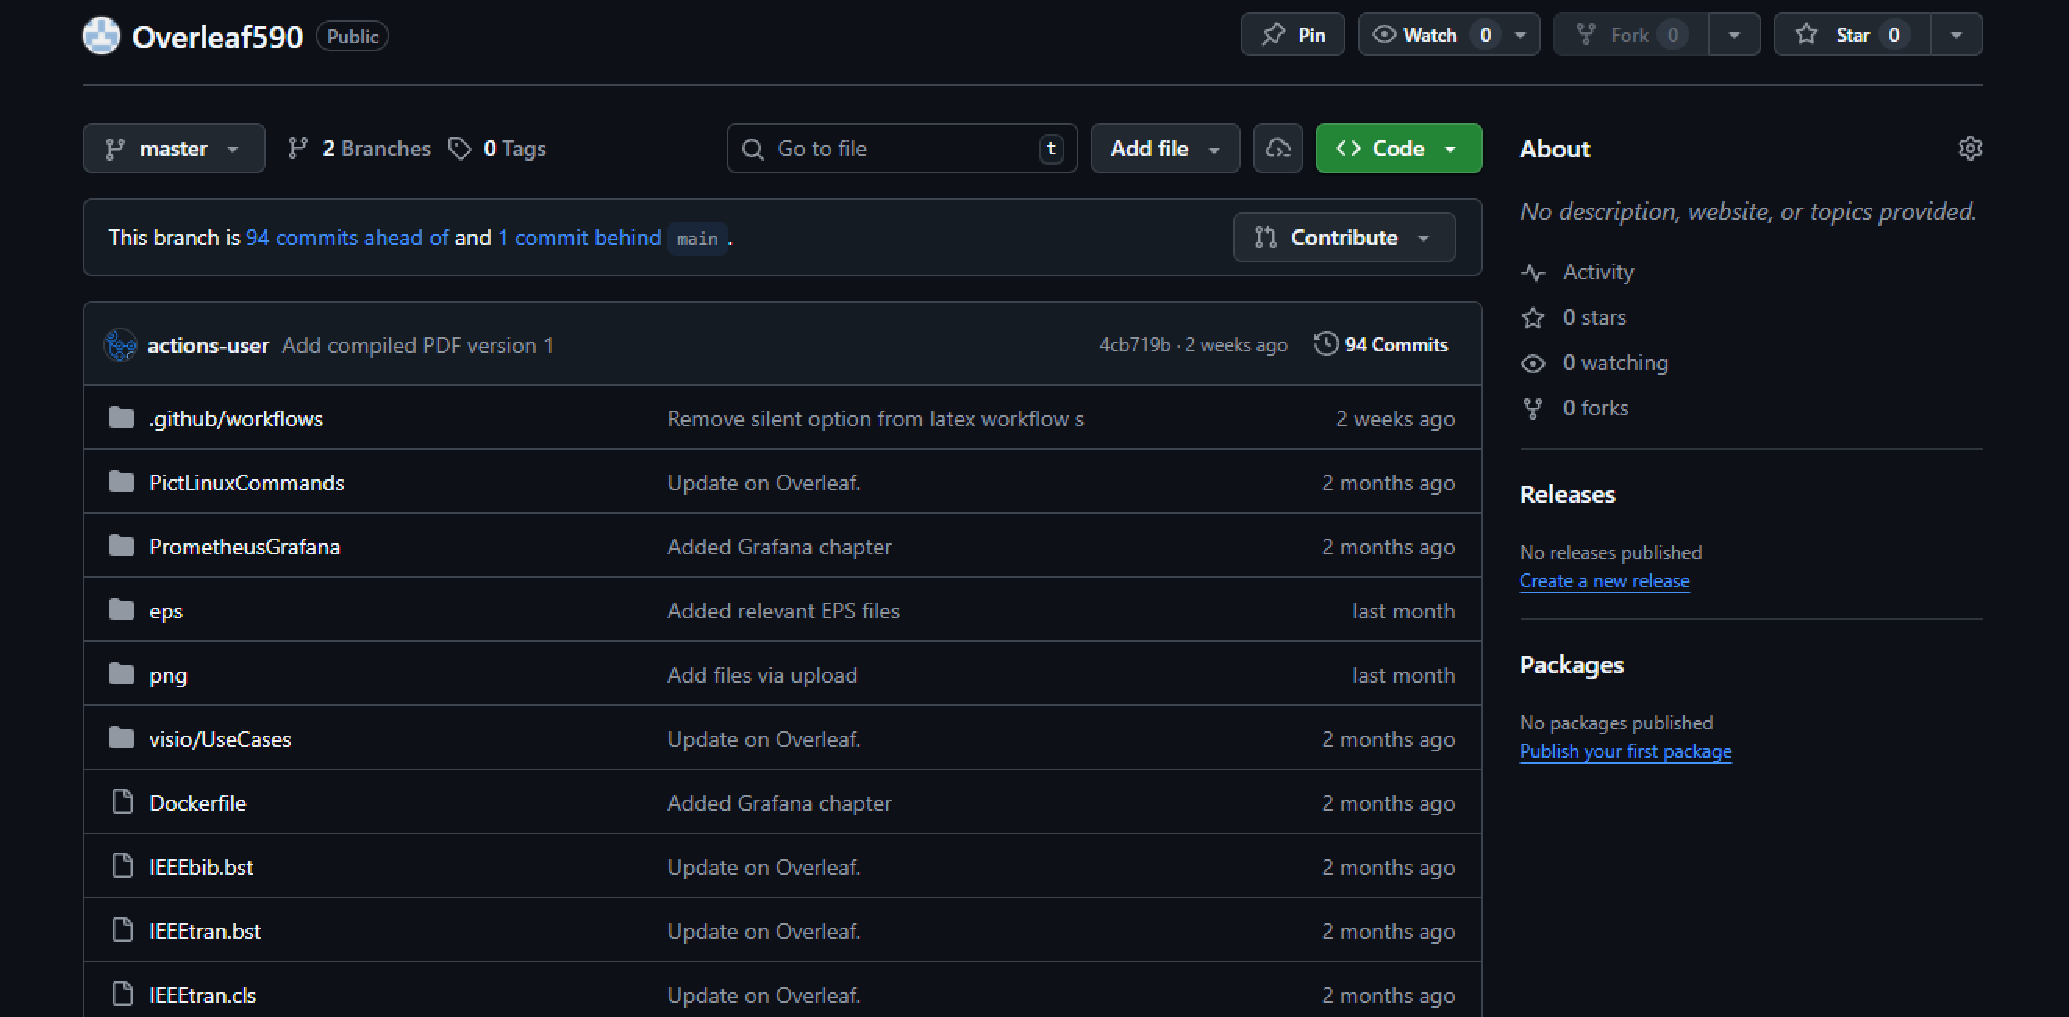
\includegraphics[width=0.9\linewidth]{pdf/b_SourceControl.pdf}
    \caption{Git Source Control}
\end{figure}

\section{Architecture Forward Documentation}

Architecture and design documentation are created and maintained using Overleaf with LaTeX. Treating documentation as source code allows it to be version-controlled, reviewed, and automatically validated. This approach supports architecture-forward development, where documentation evolves alongside implementation rather than being written after the fact.

\begin{figure}[h!]
    \centering
    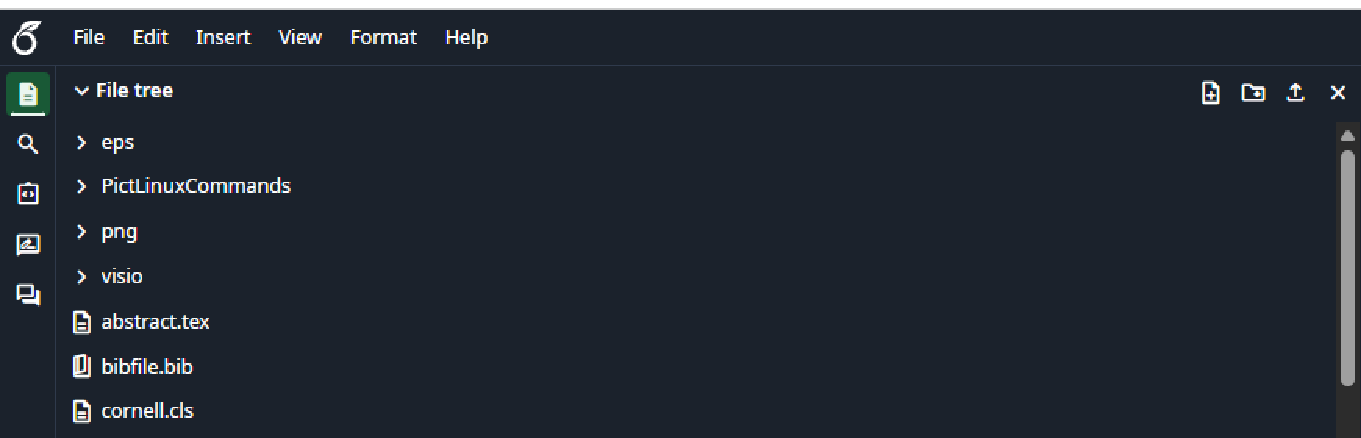
\includegraphics[width=0.9\linewidth]{pdf/c_LaTeXCompiler.pdf}
    \caption{Basic Overleaf Structure}
\end{figure}

\section{CI/CD Pipeline}

GitHub Actions is used as the CI/CD tool to orchestrate the pipeline. On every push to the \texttt{master} branch, the workflow automatically generates an appropriate PDF.

\begin{figure}[h!]
    \centering
    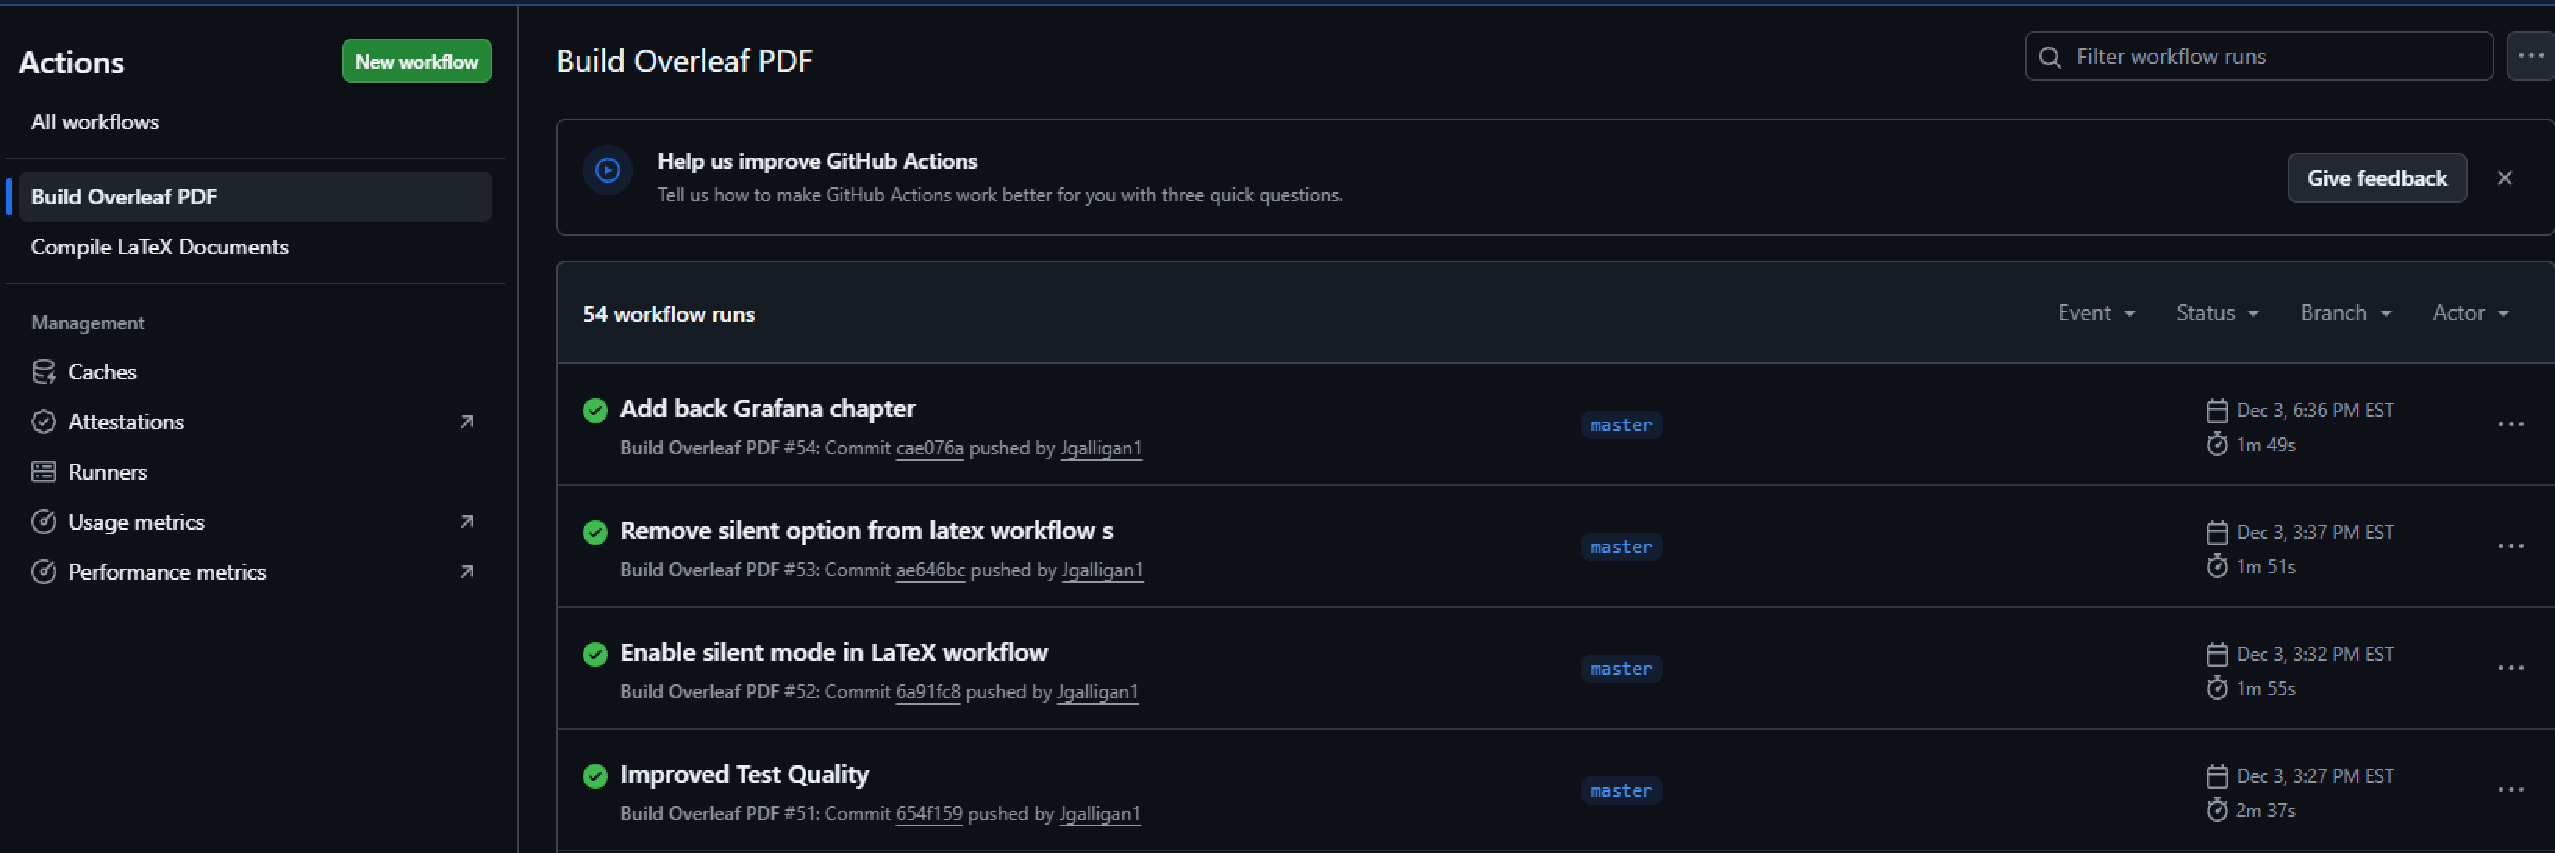
\includegraphics[width=0.9\linewidth]{pdf/d_Tools.pdf}
    \caption{CI/CD Pipeline in GitHub Actions}
\end{figure}

\section{Testing}
Our pipeline does not use a dedicated testing framework. Instead, it relies on LaTeX compilation as a form of build validation. A preliminary ‘soft compile’ functions as a smoke test, while log parsing provides basic static analysis by flagging warnings and errors.  The reason this was necessary was that telling the pipeline to ignore LaTeX warnings proved to be necessary to run the program.  The soft compile allows us to start looking for these potential errors without breaking the system.
\begin{figure}[h!]
    \centering
    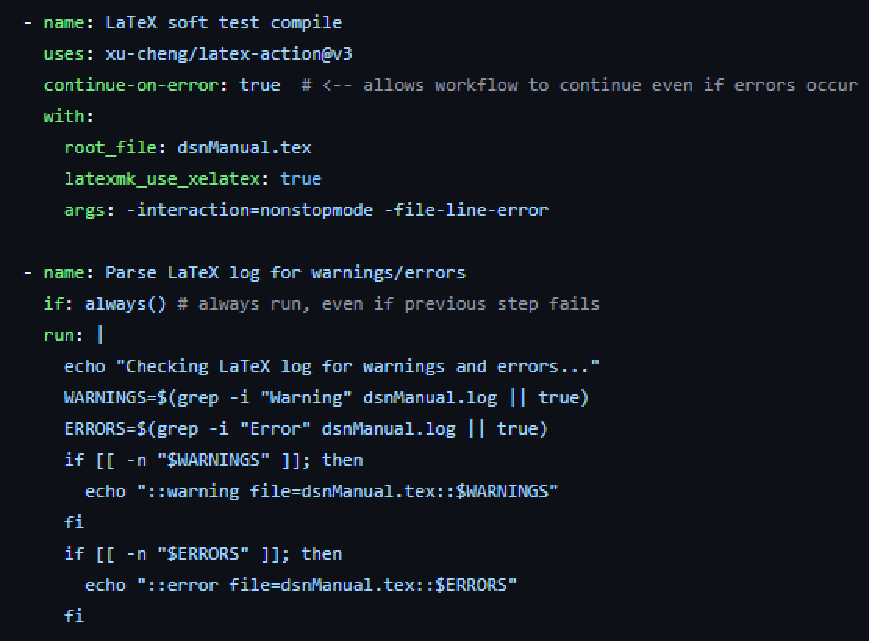
\includegraphics[width=0.9\linewidth]{pdf/e_Testing.pdf}
    \caption{Basic testing methodology}
\end{figure}

\section{Deployment}

Deployment for this project is performed using a DigitalOcean cloud server. Once the CI/CD pipeline successfully generates the compiled LaTeX documentation, the resulting PDF is deployed to the DigitalOcean environment, where it can be accessed by end users.

This deployment strategy reflects real-world DevOps practices, in which build artifacts produced by a continuous integration pipeline are delivered to a remote hosting environment. GitHub Actions is responsible for validation and artifact generation, while DigitalOcean serves as the runtime and distribution platform.

By separating the build environment from the deployment environment, the pipeline improves reliability and scalability while maintaining a lightweight and manageable infrastructure.

\section{Monitoring}
DigitalOcean is used to monitor aspects of the deployed system after deployment. Using DigitalOcean’s built-in monitoring and traffic tools, we are able to verify that requests are being received by the server and that the deployed artifacts are being accessed as expected. 

This monitoring provides basic operational feedback, allowing us to confirm that the deployment is functioning correctly without requiring a full observability stack. While lightweight, this approach is sufficient for validating system behavior and completing the monitoring phase of the DevOps pipeline.

\section{SWOT Analysis}

\begin{figure}[h!]
    \centering
    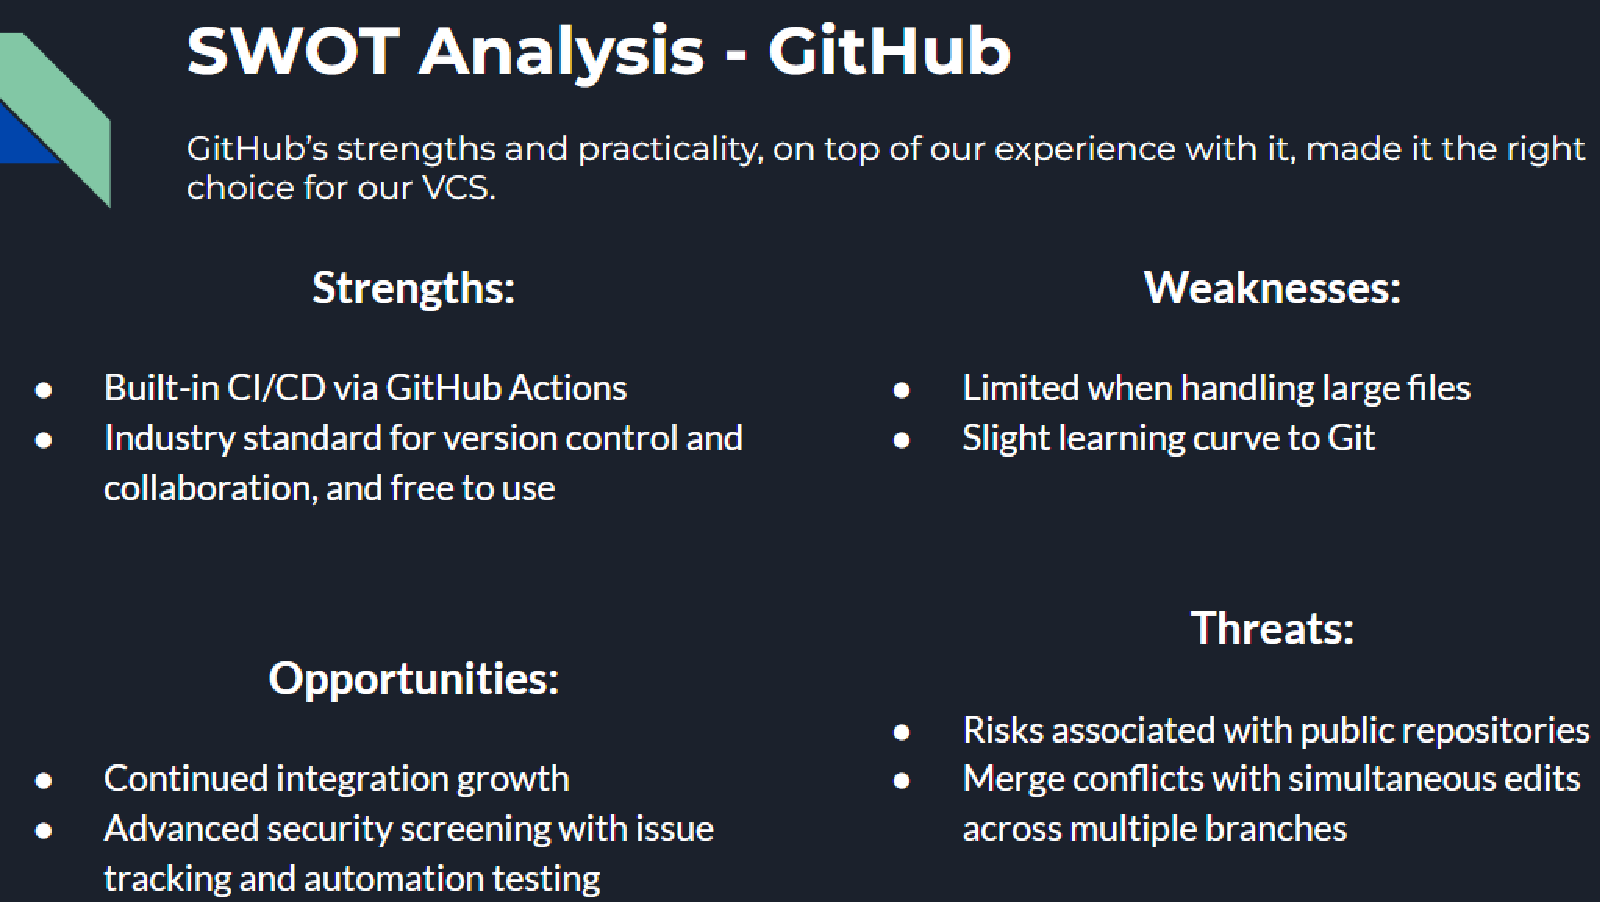
\includegraphics[width=0.9\linewidth]{pdf/SWOT_Git.pdf}
    \caption{SWOT analysis for Git}
\end{figure}

\begin{figure}[h!]
    \centering
    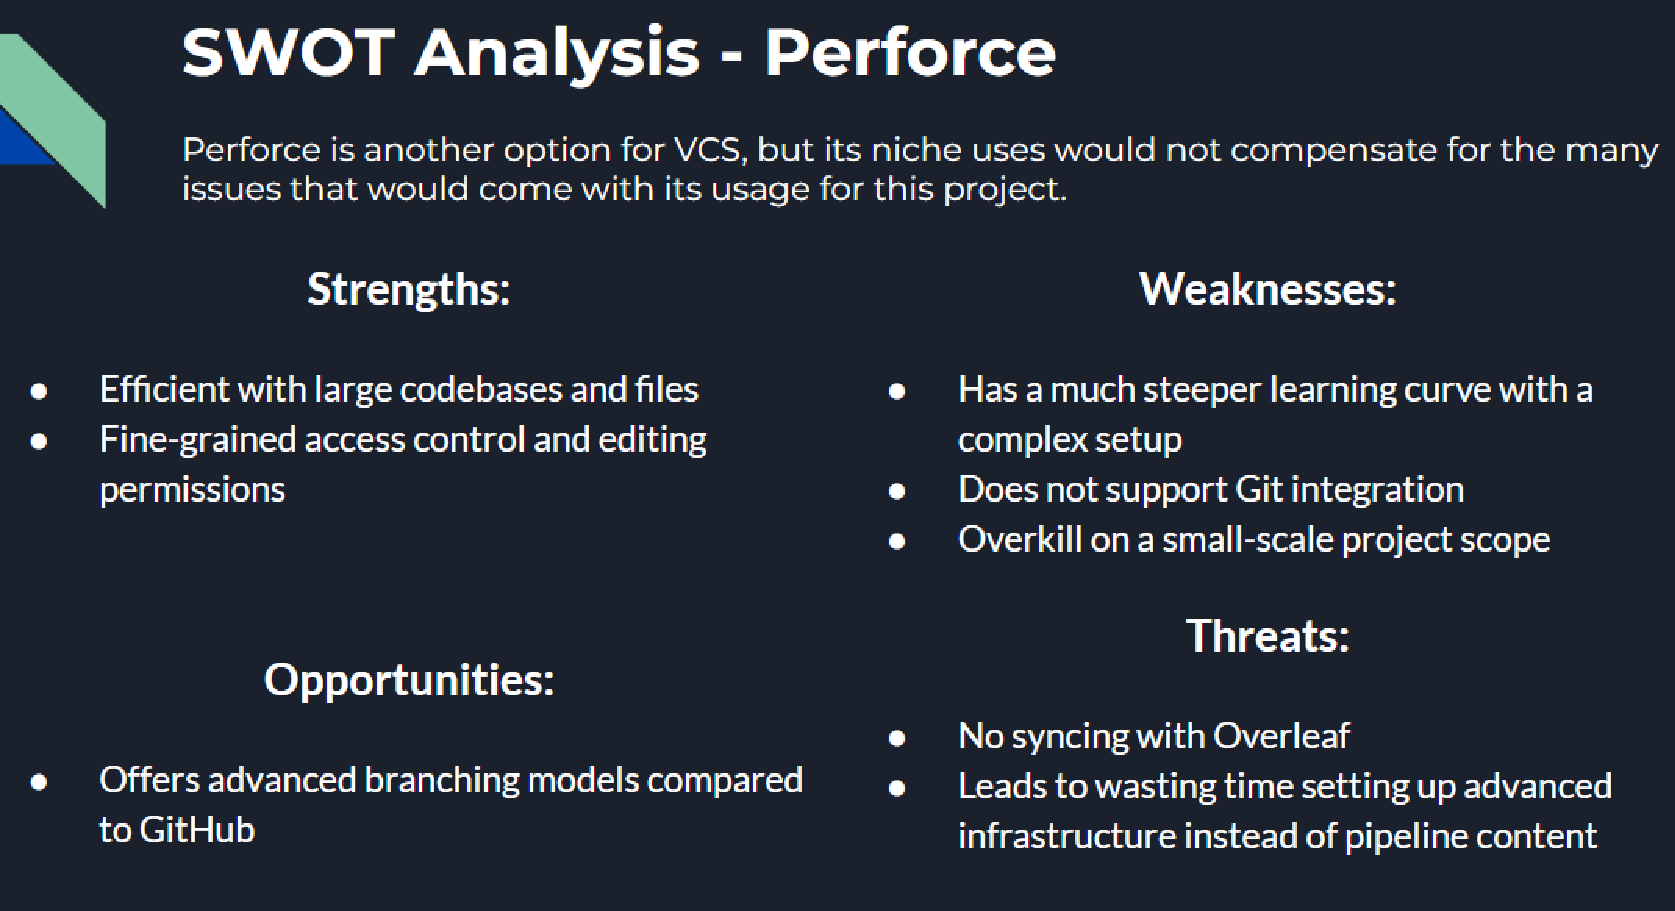
\includegraphics[width=0.9\linewidth]{pdf/SWOT_Perforce.pdf}
    \caption{Swot analysis for Perforce}
\end{figure}
